%%%%%%%%%%%%%%%%%%%%%%%%%%%%%%%%%%%%%%%%%%%%%%%%%%%%%%%%%%%%%%%%%%%
% Frontiers in Computer Science — Review article
% Class: FrontiersinHarvard (author-date reference style)
% Entry point for the Frontiers submission (conversion of ICLR v5).
%%%%%%%%%%%%%%%%%%%%%%%%%%%%%%%%%%%%%%%%%%%%%%%%%%%%%%%%%%%%%%%%%%%

\documentclass[utf8]{FrontiersinHarvard} % Harvard (author-date) — Frontiers default for most journals

\usepackage{url,hyperref,lineno,microtype,subcaption}
\hypersetup{hidelinks}
\usepackage[onehalfspacing]{setspace}
\usepackage{booktabs}
\usepackage{amssymb}
\usepackage{multirow}

\linenumbers

\graphicspath{{./}}

\def\keyFont{\fontsize{8}{11}\helveticabold }
% N5: replace the two placeholder defs below with the real author list when the
% user supplies it. \firstAuthorLast drives the running head ("Anonymous et al.").
\def\firstAuthorLast{Anonymous {et~al.}}
\def\Authors{Author 1\,$^{1,*}$, Author 2\,$^{2}$ and Author 3\,$^{1}$}
\def\Address{$^{1}$Department of Computer Science, University X, City X, Country \\
$^{2}$Department of Computer Science, University Y, City Y, Country }
\def\corrAuthor{Author 1}

\def\corrEmail{author1@example.edu}

\begin{document}
\onecolumn
\firstpage{1}

\title[Diagnostics and Infrastructure for Multi-Agent Systems]{Diagnostics and Infrastructure for Foundation Model-Based Multi-Agent Systems: A Review of the Runtime Stack}

\author[\firstAuthorLast ]{\Authors}
\address{}
\correspondance{}

\extraAuth{}

\maketitle

\begin{abstract}

\section{}
Foundation model-based multi-agent systems are rapidly deployed in production, yet the operational layers that ensure their reliability and efficiency remain fragmented. While orchestration frameworks and single-model inference optimization are well-surveyed, the diagnostics layer (failure localization, observability, safety) and the infrastructure layer (memory management, scheduling, resource allocation) for multi-agent workloads lack joint analysis. We present, to our knowledge, the first survey to jointly analyze both layers, covering 112 references and 45 systems across the diagnostics and infrastructure layers, together with 8 benchmarks. First, we construct a diagnostics taxonomy spanning three failure localization paradigms (statistical: FAMAS, 66\% top-1 accuracy; LLM-guided: TrajAudit, +24.7pp accuracy; RL-trained: AgenTracer, 69.10\% agent-level accuracy), three safety paradigms (topology-based, policy verification, ML-layered), observability standards, and failure benchmarks. Second, we identify three multi-agent workload characteristics (sparse activation, invocation distance, inter-agent memory sharing) that general serving systems do not exploit predictively, analyzed through application-aware systems spanning memory optimization (ScaleSim, up to 1.74$\times$ speedup), prefix-aware scheduling (TokenCake), cache lifecycle (Continuum), and power management (KAIROS). Third, we analyze the \emph{diagnostics--infrastructure tension}: diagnostics must retain runtime state while serving infrastructure must discard it, a conflict no surveyed system manages explicitly, and we derive four co-design opportunities from it. Claims used for cross-system comparison come from full-text sources; abstract-level results are marked \emph{[a]} and are never used to rank systems or compute deltas.

\tiny
\keyFont{ \section{Keywords:} multi-agent systems, diagnostics, failure localization, observability, safety guardrails, LLM serving, infrastructure, survey}
\end{abstract}

\section{Introduction}\label{sec:introduction}
Foundation model-based multi-agent systems (MAS), in which multiple Large Language Model (LLM) agents collaborate to solve complex tasks~\citep{metagpt2024, camel2023, chatdev2024}, have become a dominant paradigm in both research and industry. A vendor survey reports that 72\% of organizations are actively using or testing multi-agent AI systems~\citep{zapier2025} (Tier-3 vendor data, reported as stated). Systems such as MetaGPT~\citep{metagpt2024}, Internet of Agents~\citep{ioa2025}, and Graph-of-Agents~\citep{graphofagents2026} demonstrate increasing architectural sophistication. Yet this rapid deployment has outpaced reliable operational infrastructure. The gap lies in two under-explored layers of the multi-agent runtime stack: the \emph{diagnostics layer}, which provides failure localization, observability, and safety mechanisms, and the \emph{infrastructure layer}, which manages memory, scheduling, and resource allocation for multi-agent workloads.

While orchestration frameworks (LangGraph, CrewAI, AutoGen) have received substantial survey attention~\citep{zhu2026orchestration}, and single-model inference optimization is well-studied, no unifying taxonomy connects these systems~\citep{beyondindiv2026}. We count 45 systems across our own tables\footnote{Counted across our own system tables: 12 failure-localization methods, 12 observability and safety systems, and 21 infrastructure systems. Benchmarks (8) and comparator surveys (6) are excluded.}, and serving systems designed for single-model inference inadequately address multi-agent characteristics such as sparse activation and inter-agent memory sharing.

This survey bridges this gap with, to our knowledge, the first joint analysis of the diagnostics and infrastructure layers of multi-agent systems. Table~\ref{tab:surveys} contrasts our scope against six adjacent surveys. Orchestration surveys~\citep{zhu2026orchestration} cover agent interaction topologies; evaluation surveys~\citep{evalbenchmark2025, evalagents2026, llmbenchsurvey2025} measure agent quality through offline benchmarks; the AgentOps survey~\citep{agentopssurvey2025} and related operations work~\citep{agentopscsiro2024, architectingops2026} taxonomize the monitoring-to-resolution pipeline; safety surveys~\citep{safellmagentsurvey2026, trustworthyagents2025} address agent trustworthiness; and serving-latency surveys~\citep{latencysurvey2026} optimize inference latency. General agent surveys~\citep{li2024, abouali2025, wang2026classical, tran2025} cover architectural patterns and collaboration mechanisms but not the runtime operational layers. The closest are \citet{beyondindiv2026}, which surveys collaboration and failure but not infrastructure, and \citet{li2024}, whose ``infrastructure'' refers to the workflow layer rather than serving systems. None jointly treats runtime diagnostics and multi-agent infrastructure, and none compares systems quantitatively across the two layers.

Our verification strategy is described in \S\ref{sec:background}: comparative quantitative claims come from full-text sources, while abstract-level results are marked \emph{[a]} and excluded from comparisons. Figure~\ref{fig:overview} illustrates our survey scope.

\begin{table*}[t]
\centering
\caption{Comparison with existing surveys. $\bullet$ = covered, $\circ$ = not covered. $^a$A 2026 survey of MAS collaboration and failure; it organises failure conceptually and does not catalogue system-level localization methods or cover infrastructure. $^b$A 2024 survey covering workflow and architecture; its ``infrastructure'' is at that level, not multi-agent serving (memory, scheduling, cache lifecycle, power). ``Quant.'' denotes that the survey reports quantitative results for the systems it reviews, at the verification depth described in \S\ref{sec:background}; it does not imply that those numbers are compared across systems. \textbf{Pub.}: $\checkmark$ = peer-reviewed venue, $\circ$ = preprint, --- = not a publication. Pub.\ records the venue only and is not a quality judgement.}
\label{tab:surveys}
\footnotesize
\setlength{\tabcolsep}{6pt}
\begin{tabular}{@{}llcccccc@{}}
\toprule
\textbf{Survey} & \textbf{Year} & \textbf{Venue} & \textbf{Orch.} & \textbf{Diag.} & \textbf{Infra} & \textbf{Quant.} & \textbf{Pub.} \\
\midrule
Zhu et al. & 2026 & Future Internet & $\bullet$ & $\circ$ & $\circ$ & $\circ$ & $\checkmark$ \\
AgentOps & 2025 & preprint & $\circ$ & $\bullet$ & $\circ$ & $\circ$ & $\circ$ \\
Mohammadi et al. & 2025 & ACM KDD & $\circ$ & $\circ$ & $\circ$ & $\circ$ & $\checkmark$ \\
Latency survey & 2026 & IEEE Access & $\circ$ & $\circ$ & $\bullet$ & $\circ$ & $\checkmark$ \\
Qi et al.$^a$ & 2026 & preprint & $\circ$ & $\bullet$ & $\circ$ & $\circ$ & $\circ$ \\
Li et al.$^b$ & 2024 & Vicinagearth & $\circ$ & $\circ$ & $\circ$ & $\circ$ & $\checkmark$ \\
\textbf{Ours} & 2026 & --- & $\circ$ & $\bullet$ & $\bullet$ & $\bullet$ & --- \\
\bottomrule
\end{tabular}
\end{table*}

\begin{figure*}[t]
\centering
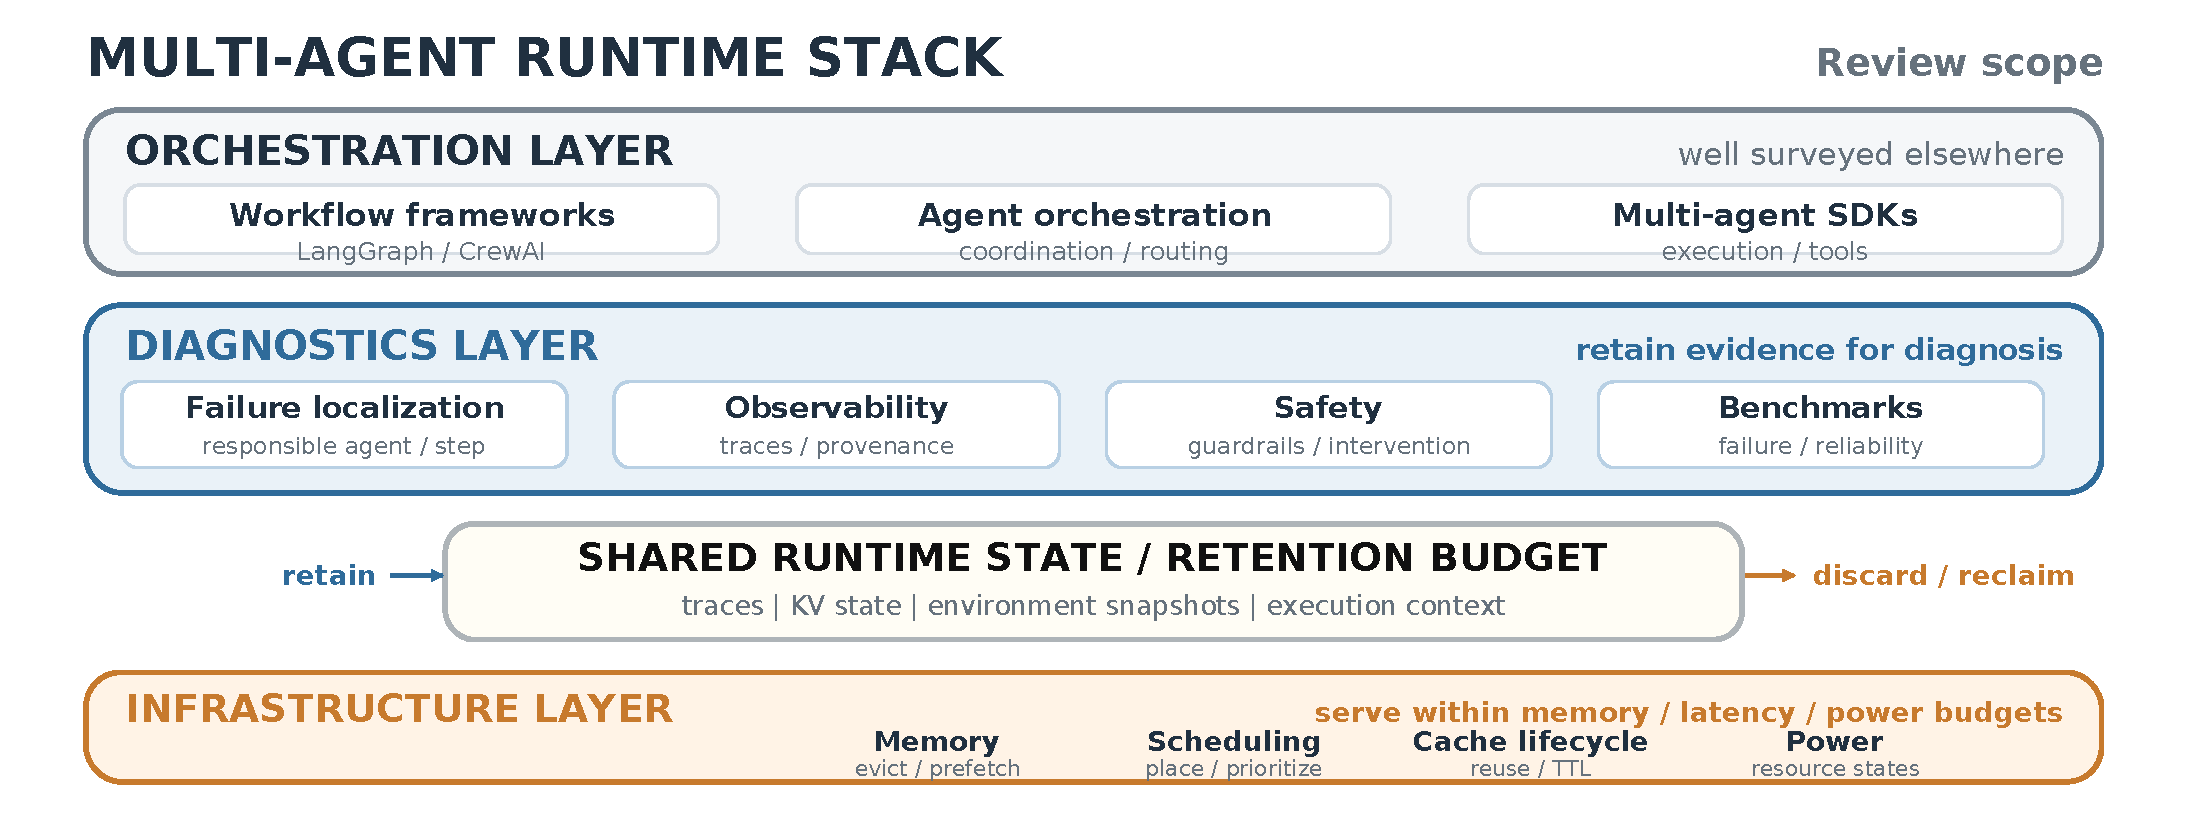
\includegraphics[width=\textwidth]{fig1_overview.pdf}
\caption{Survey scope: the multi-agent runtime stack. Our survey covers the diagnostics layer (\S\ref{sec:diagnostics}) and the infrastructure layer (\S\ref{sec:infrastructure}); the orchestration layer (top, dashed) is well-covered by existing surveys. The two-way arrow marks the retention tension analyzed in \S\ref{sec:tension}, which connects the two layers.}
\label{fig:overview}
\end{figure*}

Our contributions are:
\begin{enumerate}
\item \textbf{Diagnostics taxonomy.} We organize multi-agent diagnostics into four subcategories spanning failure localization (\S\ref{sec:diag_fl}), observability (\S\ref{sec:diag_obs}), safety (\S\ref{sec:diag_safety}), and benchmarks (\S\ref{sec:diag_bench}), covering three failure localization paradigms (statistical, LLM-guided, RL-trained) and three safety paradigms (topology-based, policy verification, ML-layered).
\item \textbf{Infrastructure challenge analysis.} We identify three multi-agent workload characteristics (sparse activation, invocation distance, inter-agent memory sharing) that existing single-LLM serving systems do not exploit predictively, demonstrated through application-aware systems spanning memory optimization (ScaleSim, up to 1.74$\times$ speedup~\citep{zhou2026}), prefix-aware scheduling (TokenCake~\citep{tokencake2025}), cache lifecycle (Continuum), and power management (KAIROS).
\item \textbf{Cross-layer tension analysis.} We identify and analyze the fundamental conflict between the two layers, namely that diagnostics must \emph{retain} runtime state while serving infrastructure must \emph{discard} it, and derive four co-design opportunities from this tension rather than listing them in isolation (\S\ref{sec:tension}, with the opportunities developed in \S\ref{sec:discussion}).
\end{enumerate}

\section{Background}\label{sec:background}
A foundation model-based agent operates in a perception-reasoning-action loop, using an LLM to process observations and execute actions (tool invocations, code execution, inter-agent communication). A multi-agent system (MAS) comprises multiple such agents, as exemplified by MetaGPT~\citep{metagpt2024}, CAMEL~\citep{camel2023}, ChatDev~\citep{chatdev2024}, and IoA~\citep{ioa2025}, operating within a shared environment or communicating to accomplish collective objectives~\citep{li2024, wang2026classical}. MAST~\citep{mast2025} identifies 14 recurring failure patterns in such systems. These failures motivate systematic diagnostics.

Multi-agent systems introduce three characteristics relevant to this survey~\citep{understandingmas2026}: (1)~\emph{distributed execution} across concurrent agents requiring coordination of LLM requests; (2)~\emph{inter-agent communication} creating complex traces that span agent boundaries, where failures cascade through communication channels~\citep{famas2025, traceelephant2026}; and (3)~\emph{inter-agent memory sharing}, where agents reuse prompts, tools, and cached state across the system. This last property, together with sparse activation, creates memory management challenges beyond single-model serving~\citep{zhou2026, kvcachesurvey2026}.

\paragraph*{Scope and verification procedure.} We focus on runtime operational layers distinct from three well-surveyed areas: orchestration~\citep{zhu2026orchestration}, single-model inference~\citep{kwon2023}, and offline evaluation~\citep{evalbenchmark2025}. Because we report numbers, we need an explicit rule for how far each number was checked rather than a closed list of trusted papers. We assign every cited system to a tier by the following procedure, applied in order:

\begin{enumerate}
\item \textbf{Tier 1a (full-text verified).} The source was read in full and the specific quantitative claim was located in the body text or a table. These numbers may be compared and quoted.
\item \textbf{Tier 1b (read in full, not page-verified).} The source was read in full and has a confirmed peer-reviewed venue, but the quantitative claim was taken from the published text without being cross-checked against a specific page, table, or figure. These numbers may be quoted with the $^\dagger$ marker but are not used to compute cross-system deltas.
\item \textbf{Tier 2 (abstract-only).} Only the abstract was read; the body was not examined. This applies to preprints and workshop papers, and equally to venue-published papers whose body we did not read. The claim is reported as stated and marked \emph{[a]}. The distinction from Tier 1b is therefore how much of the source was read, not the standing of its venue: Tier 1b means the full text was read, Tier 2 means it was not.
\item \textbf{Tier 3.} Documentation, platform pages, and vendor reports, labelled by source type and used for context only.
\end{enumerate}

Applying this procedure yields \textbf{8 Tier-1 papers across 9 table entries: 5 in Tier~1a} (FAMAS, TrajAudit, Agent Traces, TraceElephant, ScaleSim) and \textbf{3 in Tier~1b} (G-Safeguard at ACL 2025, ShieldAgent at ICML 2025, and AgenTracer at ICLR 2026). RootSE is the benchmark introduced by TrajAudit, so the two rows share one paper. Systems such as RAFFLES, AgentLocate, MultiAgentBench, and Who\&When do have confirmed venues but were read at abstract level, which under the procedure above places them in Tier~2, not Tier~1; the tier reflects verification depth rather than the standing of the venue. LlamaFirewall is likewise Tier~2: it is distributed as a preprint and was read at abstract level.

\section{Diagnostics Layer}\label{sec:diagnostics}
This section presents our taxonomy of multi-agent diagnostics, organized into four subcategories: failure localization (Section~\ref{sec:diag_fl}), observability (Section~\ref{sec:diag_obs}), safety (Section~\ref{sec:diag_safety}), and benchmarks (Section~\ref{sec:diag_bench}). Figure~\ref{fig:taxonomy} maps the landscape of diagnostic functions and representative systems, whereas Figure~\ref{fig:pipeline} provides a complementary process view showing where tracing, localization, root-cause output, and safety act along execution.

\begin{figure*}[t]
\centering
\includegraphics[width=0.8\textwidth]{figures/figure2.png}
\caption{Landscape of multi-agent diagnostics across four subcategories. Stars ($\star$) mark Tier~1 systems (Tier~1a or 1b); unmarked leaves are Tier~2 (abstract-verified) or, for standards and tooling, Tier~3. The tier rule and the 1a/1b split are given in Section~\ref{sec:background}.}
\label{fig:taxonomy}
\end{figure*}

\subsection{Failure Localization}\label{sec:diag_fl}

When a multi-agent system fails, identifying the responsible agent and faulty action remains a central challenge. Our surveyed set contains twelve failure-localization methods from 2024--2026. We group them into three recurring paradigms---statistical, LLM-guided, and RL-trained---that use distinct methodological assumptions and evaluation conventions. These paradigms differ along two axes: \emph{input requirements} (replay-based vs.\ single-execution) and \emph{attribution granularity} (agent-level, step-level, or action-level). Table~\ref{tab:failure_loc} summarizes the landscape.

\paragraph*{Statistical approaches}
These methods apply spectrum-based fault localization (SBFL) to multi-agent traces. FAMAS~\cite{famas2025} replays trajectories $k=20$ times and applies four suspiciousness metrics (action coverage, failure entropy, temporal decay, Kulczynski2), achieving 66\% top-1 action-level accuracy on the 82-failure replayable subset of Who\&When~\cite{famas2025}. Complementary statistical methods extend SBFL without replays: CausalFlow~\cite{flatlogs2026} constructs hierarchical causal graphs (36.2\% step accuracy, abstract-verified) and StepFinder~\cite{stepfinder2026} applies temporal semantic analysis (+10.35pp, abstract-verified). Zero-replay debugging~\cite{zeroreplay2026} eliminates replay overhead entirely through knowledge-based reasoning (abstract-verified).

\paragraph*{LLM-guided approaches}
These treat diagnosis as a reasoning task. TrajAudit~\cite{trajaudit2026} deploys an LLM investigator with Semantic Saliency Folding (SSF, 86--92\% token reduction) and Prior Failure Reasoning (PFR), achieving +24.7pp step-level accuracy on RootSE (93 failures); ablation confirms SSF as critical ($-$11.4\% vs.\ $-$3.5\% for PFR)~\cite{trajaudit2026}. The LLM-guided family has rapidly diversified: AgentRx~\cite{agentrx2026} provides domain-agnostic diagnosis (+23.6pp step, +22.9pp category accuracy), TRAIL~\cite{trail2025} combines trace reasoning with issue localization, RAFFLES~\cite{raffles2026} applies reasoning-based attribution (EACL 2026), and AgentLocate~\cite{agentlocate2026} adds multi-perspective verification. Hierarchical approaches~\cite{hierrerror2025} decompose errors across agent boundaries, while VerifyMAS~\cite{verifymas2026} introduces hypothesis verification for attribution (all abstract-verified).

\paragraph*{RL-trained approaches}
These replace hand-designed metrics with learned attribution. AgenTracer~\cite{agentracer2026} trains an 8B-parameter failure tracer via reinforcement learning, achieving 69.10\% agent-level accuracy on Who\&When (184 failures), outperforming DeepSeek-R1 by 12.21pp (ICLR 2026)~\cite{agentracer2026}. MASPrism~\cite{masprism2026} takes a lightweight alternative, using a prefill-stage SLM for attribution (abstract-verified).

\paragraph*{Beyond attribution.}
Several methods extend failure localization toward repair and intervention: diagnosis-driven automatic repair~\cite{diagrepair2026} closes the loop from attribution to fix, AgentTether~\cite{agenttether2026} combines graph-guided diagnosis with runtime intervention, and interactive debugging~\cite{interactivedebug2025} enables human-in-the-loop steering (CHI 2025). Additional methods include FALAT~\cite{falat2026} (dependency-guided search), DoVer~\cite{dover2026} (intervention + replay, recovering 18--28\% of failed trials), EAGER~\cite{eager2026} (unsupervised contrastive trace representation), and holistic evaluation frameworks~\cite{holisticeval2026} (all abstract-verified). Meta-evaluation work~\cite{whwhpro2026} has begun assessing the attribution methods themselves, and the same shift toward online auditing appears in AgentForesight~\cite{agentforesight2026}, which monitors a trajectory while it runs and emits an alarm before the failure surfaces rather than reconstructing it afterwards (abstract-verified).

\begin{table*}[t]
\centering
\caption{Failure localization methods for multi-agent systems. Tier~1 results are from full-text verification, except those marked $^\dagger$, which are venue-published but reported from the published text without page-level cross-verification (Tier~1b); Tier~2 results marked [a] are as reported in source abstracts and are not independently verified. The tier rule and the 1a/1b split are given in Section~\ref{sec:background}. \textbf{Pub.}: $\checkmark$ = peer-reviewed main-track venue, $\circ$ = preprint or workshop paper. --- = not stated in the source. \emph{These numbers come from different benchmarks, protocols, and observability settings; this table is a landscape summary, not a head-to-head comparison (see Section~\ref{sec:tension}).}}
\label{tab:failure_loc}
\scriptsize
\setlength{\tabcolsep}{2pt}
\begin{tabular}{@{}p{0.145\textwidth}p{0.155\textwidth}lp{0.115\textwidth}p{0.125\textwidth}p{0.135\textwidth}cp{0.04\textwidth}@{}}
\toprule
\textbf{System} & \textbf{Approach} & \textbf{Gran.} & \textbf{Bench.} & \textbf{Overhead} & \textbf{Key Result} & \textbf{Tier} & \textbf{Pub.} \\
\midrule
FAMAS & Stat. (SBFL) & Action & Who\&When & 20 replays & 66\% top-1 & 1 & $\circ$ \\
TrajAudit & LLM-guided & Step & RootSE & 86--92\% tok. & +24.7pp & 1 & $\circ$ \\
AgenTracer & RL (8B) & Agent & Who\&When & 8B train & 69.10\% & 1$^\dagger$ & $\checkmark$ \\
AgentRx & LLM-guided & Step & --- & --- & +23.6pp step [a] & 2 & $\circ$ \\
FALAT & Dependency & Step & Who\&When & --- & 46.0\% step [a] & 2 & $\circ$ \\
DoVer & Interv.+Replay & Step & --- & multiple replays & 18--28\% [a] & 2 & $\checkmark$ \\
MASPrism & Prefill SLM & Step & --- & --- & --- [a] & 2 & $\circ$ \\
RAFFLES & Reasoning & Step & Who\&When & --- & --- [a] & 2 & $\checkmark$ \\
AgentLocate & LLM judge & Step & --- & --- & --- [a] & 2 & $\checkmark$ \\
CausalFlow & Stat. (Causal) & Step & --- & --- & 36.2\% [a] & 2 & $\circ$ \\
StepFinder & Temporal sem. & Step & Who\&When & --- & +10.35pp [a] & 2 & $\circ$ \\
EAGER & Contrastive & System & --- & --- & prelim. [a] & 2 & $\circ$ \\
\bottomrule
\end{tabular}
\end{table*}
\vspace{-2pt}
{\footnotesize \emph{Non-comparability.} The ``Key Result'' column aggregates measurements taken on different benchmarks (Who\&When, RootSE, or task-specific sets), under different observability settings (output-only vs.\ full traces), and against different baselines. Methods also differ in what they require at inference time (replay budget, training, token cost). The rows therefore describe a landscape of approaches, not a ranked comparison; no cross-row ranking should be inferred. Pub.\ records the publication venue only and is not a quality judgement.}

\subsection{Observability and Tracing}\label{sec:diag_obs}

Failure localization depends on rich execution traces, yet the multi-agent observability stack remains fragmented across three levels: conceptual models, protocols, and tooling~\cite{aiobsmultilayer2026}.

At the \emph{conceptual level}, \cite{agenttraces2026} present a seven-dimension provenance taxonomy (trace sources, evidence units, execution units, nine relation types, run-to-token granularity, online/offline timing, interaction context). This taxonomy exposes a key architectural split between post-hoc debugging and runtime enforcement. Complementary taxonomies address observability from an operations perspective~\cite{agentopscsiro2024, architectingops2026, agentsysops2026}, and a multi-layer survey~\cite{aiobsmultilayer2026} proposes a five-layer framework spanning data, model, agent, system, and application observability (all abstract-verified).

At the \emph{protocol level}, the OpenTelemetry GenAI conventions~\cite{opentelemetry2026} provide vendor-neutral attributes (\texttt{gen\_ai.*}) for LLM spans, but semantic interoperability remains limited. AgentTrace~\cite{agenttrace2026} proposes structured logging specifically for agent systems (AAAI 2026 Workshop, abstract-verified), and process mining approaches~\cite{processobserv2025} apply workflow analysis to agent traces (abstract-verified).

At the \emph{tooling level}, a vendor survey reports 89\% observability adoption among enterprises using AI agents~\cite{zapier2025} (Tier-3 vendor data), with LangSmith~\cite{langsmith2026}, Langfuse, and Arize Phoenix as leading platforms. The Insights Generator~\cite{insightsgenerator2026} demonstrates that corpus-level trace mining improves downstream performance by 30.4pp (abstract-verified). Security-focused tooling has also emerged: auditable agent frameworks~\cite{auditableagents2026, secaudit2026} build unified graphs for security auditing, and view-oriented compilers~\cite{viewcompiler2026} enable multi-perspective trace analysis (all abstract-verified).

Table~\ref{tab:obs_safety} summarizes the observability and safety landscape.

\begin{table*}[t]
\centering
\caption{Observability, tracing, and safety systems. \textbf{Pub.}: $\checkmark$ = peer-reviewed main-track venue, $\circ$ = preprint, workshop paper, or no confirmed venue, --- = documentation or platform (not a publication). Pub.\ records the venue only and is not a quality judgement.}
\label{tab:obs_safety}
\footnotesize
\setlength{\tabcolsep}{5pt}
\begin{tabular}{@{}llccc@{}}
\toprule
\textbf{System} & \textbf{Category} & \textbf{Open} & \textbf{Tier} & \textbf{Pub.} \\
\midrule
\multicolumn{5}{l}{\emph{Observability \& Tracing}} \\
Agent Traces & Taxonomy & --- & 1 & $\circ$ \\
OTel GenAI & Standard & \checkmark & 3 & --- \\
AgentTrace & Structured log & --- & 2 & $\circ$ \\
LangSmith & Platform & --- & 3 & --- \\
Insights Gen. & Diagnostic & --- & 2 & $\circ$ \\
\midrule
\multicolumn{5}{l}{\emph{Safety \& Reliability}} \\
G-Safeguard & Topology GNN & --- & 1$^\dagger$ & $\checkmark$ \\
ShieldAgent & Policy verif. & --- & 1$^\dagger$ & $\checkmark$ \\
LlamaFirewall & ML-layered & \checkmark & 2 & $\circ$ \\
SAIGuard & Proactive MAS & --- & 2 & $\circ$ \\
AGrail & Lifelong guard & --- & 2 & $\circ$ \\
AgentDoG & Alignment & --- & 2 & $\circ$ \\
ReGuard & Reactive & --- & 2 & $\circ$ \\
\bottomrule
\end{tabular}
\par\vspace{2pt}{\footnotesize $^\dagger$Venue-published; not page-level verified.}
\end{table*}

\subsection{Safety and Reliability}\label{sec:diag_safety}

Multi-agent safety poses a distinct challenge: attacks propagate through inter-agent communication, so a single compromised agent can corrupt downstream outputs~\cite{safellmagentsurvey2026, trustworthyagents2025}. Recent surveys identify this cross-agent propagation as the defining difference from single-agent safety~\cite{fullstacksafety2025}. Three paradigms have emerged, each at a different abstraction level. We follow the literature's convention of treating safety as a diagnostic subcategory; as Section~\ref{sec:discussion} argues, this placement is contestable, because a guardrail must both inspect state and act on the serving path.

\emph{Topology-based} approaches exploit the communication graph. G-Safeguard~\cite{gsafeguard2025} uses a GNN to detect anomalies on the multi-agent utterance graph and applies topological intervention, recovering over 40\% of the performance lost to prompt injection (ACL 2025; Tier 1b). SAIGuard~\cite{saiguard2026} extends this to communication-state simulation for proactive defense, SentinelAgent~\cite{sentinelagent2025} detects node-, edge-, and path-level anomalies on a typed execution graph, and BlindGuard~\cite{blindguard2025} performs the same detection without attack labels by training on normal-only interaction data (all abstract-verified). This graph-level reasoning is particularly salient in multi-agent settings because failures can propagate across inter-agent communication edges.

\emph{Policy-reasoning guardrails} verify another agent's action trajectory against explicit safety policies. ShieldAgent~\cite{shieldagent2025} is a single guardrail agent that extracts verifiable rules from policy documents and checks each proposed action against them, reporting 90.1\% recall of violated rules while using 64.7\% fewer API queries and 58.2\% less inference time than prior approaches (ICML 2025; Tier~1b). \cite{probabilisticarchitecture2026} provide a theoretical foundation via a three-layer probabilistic architecture, and VeriGuard~\cite{veriguard2025} applies verified code generation for safety-critical agents. The Swiss Cheese model~\cite{swisscheese2025} offers a complementary defense-in-depth framework (all abstract-verified).

\emph{ML-layered} defenses stack classifiers. LlamaFirewall~\cite{llamafirewall2025} layers PromptGuard2 (AUC 0.98) with an alignment verifier, reducing attack success from 17.6\% to 1.75\%. AGrail~\cite{agrail2025} introduces lifelong adaptive guardrails that evolve with agent deployment (abstract-verified), and GuardAgent~\cite{guardagent2024} enables knowledge-based guardrail reasoning (abstract-verified).

Complementary systems span pre-execution alignment (AgentDoG~\cite{agentdog2026}), control-theoretic recovery (ReGuard~\cite{pandya2025}), and automated auditing (AgentAuditor~\cite{agentauditor2025}, NeurIPS 2025). Safety benchmarks include GuardianAgentBench~\cite{guardianagentbench2026} (580 scenarios), OSGuard~\cite{osguard2026} (2.7\% FPR), Agent-SafetyBench~\cite{agentsafetybench2024}, and AgentHarm~\cite{agentharm2024} (all abstract-verified).

\subsection{Benchmarks}\label{sec:diag_bench}

Progress in diagnostics depends on benchmarks varying in failure coverage, trace fidelity, and evaluation scope. Table~\ref{tab:benchmarks} summarizes the landscape.

The highest-fidelity benchmark is TraceElephant~\cite{traceelephant2026}: 220 failures from three production systems with full observability. At the \emph{agent} level, complete traces raise attribution accuracy from 51\% for output-only logs to 62.2\% (+11.2pp, a 22\% relative gain), both under the same All-at-Once protocol. At the \emph{step} level, the same comparison raises accuracy from 16\% to 28.1\% (+12.1pp, a 76\% relative gain), i.e.\ step-level attribution is substantially more sensitive to missing information than agent-level attribution~\cite{traceelephant2026}. Who\&When~\cite{whenwhen2025} provides 184 failures from 127 multi-agent systems as the first dedicated failure attribution benchmark, now with a meta-evaluation extension~\cite{whwhpro2026} (abstract-verified). Domain-specific, RootSE~\cite{trajaudit2026} offers 93 SWE-bench failures with step-level annotations.

Beyond failure attribution, ReliabilityBench~\cite{reliabilitybench2026} reveals that pass@1 overestimates reliability by 20--40\% (abstract-verified), BenchGuard~\cite{benchguard2026} audits benchmark quality (abstract-verified), and MultiAgentBench~\cite{multiagentbench2025} evaluates multi-agent collaboration (ACL 2025, abstract-verified). Safety-specific benchmarks include Agent-SafetyBench~\cite{agentsafetybench2024}, AgentHarm~\cite{agentharm2024}, Agent Security Bench~\cite{asb2025} (ICLR 2025, which reports attack success above 84\% with existing defenses barely effective), and TAMAS~\cite{tamas2026} (ACL 2026, covering Byzantine, colluding, and contradicting agents) (all abstract-verified). A unified capabilities framework~\cite{unifiedcapab2026} and a benchmarking survey~\cite{evalbenchmark2025} address the meta-question of what benchmarks should measure.

\begin{table*}[t]
\centering
\caption{Diagnostics and safety benchmarks. \textbf{Pub.}: $\checkmark$ = peer-reviewed venue, $\circ$ = preprint / no confirmed venue. Pub.\ records the venue only and is not a quality judgement.}
\label{tab:benchmarks}
\footnotesize
\setlength{\tabcolsep}{5pt}
\begin{tabular}{@{}lccccc@{}}
\toprule
\textbf{Benchmark} & \textbf{Scale} & \textbf{Traces} & \textbf{Domain} & \textbf{Tier} & \textbf{Pub.} \\
\midrule
TraceElephant & 220 & Full & Multi & 1 & $\circ$ \\
Who\&When & 184 & Output & Multi & 2 & $\checkmark$ \\
RootSE & 93 & Full & SWE & 1 & $\circ$ \\
MultiAgentBench & --- & --- & Collab & 2 & $\checkmark$ \\
Agent-SafetyBench & --- & --- & Safety & 2 & $\circ$ \\
AgentHarm & --- & --- & Safety & 2 & $\circ$ \\
ReliabilityBench & --- & --- & Reliab. & 2 & $\circ$ \\
BenchGuard & --- & --- & Meta & 2 & $\circ$ \\
\bottomrule
\end{tabular}
\end{table*}

Among the benchmarks surveyed here, none evaluates diagnostics--infrastructure interaction: how diagnostic overhead affects serving performance, or how retention and serving policies affect diagnostic fidelity.

\paragraph*{Diagnostics synthesis.} Across the four diagnostic subcategories, the common dependency is retained execution evidence: localization methods require traces or replays, observability determines what evidence exists, and safety mechanisms must inspect enough context to intervene. The literature is broad but methodologically heterogeneous, so the taxonomy is most useful for comparing assumptions---trace fidelity, replay budget, granularity, and intervention timing---rather than headline accuracy across rows. This shared dependence on runtime evidence motivates the retention analysis in Section~\ref{sec:tension}.

\begin{figure*}[t]
\centering
\includegraphics[width=0.8\textwidth]{figures/figure3.png}
\caption{Process view of multi-agent diagnostics. Execution traces are collected through observability infrastructure, then processed through failure localization to produce root-cause attribution, while safety mechanisms may operate continuously alongside execution. This figure complements the landscape in Figure~\ref{fig:taxonomy}: it shows when diagnostic functions act rather than reclassifying the systems.}
\label{fig:pipeline}
\end{figure*}


\section{Infrastructure Layer}\label{sec:infrastructure}
Existing LLM serving systems were designed for single-model inference and address multi-agent workloads only partially. We identify three such challenges (\S\ref{sec:infra_challenges}), analyze application-aware systems that exploit them (\S\ref{sec:infra_scalesim}), and survey the broader landscape (\S\ref{sec:infra_landscape}).

\subsection{Multi-Agent Serving Challenges}\label{sec:infra_challenges}

Single-model serving systems (vLLM~\citep{kwon2023}, SGLang~\citep{sglang2024}, DistServe~\citep{distserve2024}) serve each request largely independently, though peer-reviewed work has begun to expose application structure: Parrot~\citep{parrot2024} passes an application-level dependency graph (semantic variables) to the scheduler, Preble~\citep{preble2025} optimizes distributed prompt sharing, Sarathi-Serve~\citep{sarathi2024} introduces chunked prefill, InferCept~\citep{infercept2024} retains KV state across tool-call interruptions, and S-LoRA~\citep{slora2024} and dLoRA~\citep{dlora2024} serve many concurrent adapters. These systems approach multi-agent serving from the general side; we return to how they differ from agent-native designs in \S\ref{sec:tension}. A recent KV cache management survey~\citep{kvcachesurvey2026} confirms that multi-agent workloads violate the per-request assumption in three ways.

\textbf{Sparse activation.} Only a fraction of agents invoke the LLM at any moment: a 1,000-agent simulation may have fewer than 10 actively generating tokens~\citep{zhou2026}. GPU memory allocated to inactive agents is wasted under conventional policies.

\textbf{Invocation distance.} Many workloads have predictable activation patterns such as sequential queues, event-driven messaging, and dependency graphs. The temporal gap before an agent's next call, termed \emph{invocation distance}~\citep{zhou2026}, is estimable from application semantics but invisible to general-purpose schedulers.

\textbf{Inter-agent memory sharing.} Agents share context (system prompts, environment descriptions, tool schemas), and general serving systems already reuse such prefixes once they appear: SGLang's RadixAttention and vLLM's automatic prefix caching both do this. What they cannot do is anticipate the \emph{application layer's} future call structure (dependency graph, message queue, execution order), so they can neither prefetch predictively nor evict semantically. This is the gap multi-agent systems target through predictive prefix management: TokenDance~\citep{tokendance2026} proposes collective KV-cache sharing across agents, DroidSpeak~\citep{droidspeak2024} enables cache reuse across different model variants, KVFlow~\citep{kvflow2025} exploits an agent step graph to evict workflow-aware and prefetch ahead of the predicted next call, and KVCOMM~\citep{kvcomm2025} aligns cache offsets across divergent per-agent prefixes so that cross-agent reuse survives the prefix change (all abstract-verified). Persistent agent-memory systems (for example A-MEM and the Mesh Memory Protocol) address a related but distinct problem, long-term memory representation rather than serving-time cache reuse, and are outside our scope.

\subsection{Application-Aware Serving}\label{sec:infra_scalesim}

Recent systems demonstrate that exploiting multi-agent workload structure yields substantial gains across four optimization axes: memory optimization, prefix-aware scheduling, cache lifecycle, and power management.

\paragraph*{Memory optimization via invocation distance.}
ScaleSim~\citep{zhou2026} introduces invocation distance as a first-class scheduling primitive. Two mechanisms exploit predictions: \emph{proactive prefetching} loads agent states before they are needed, and \emph{distance-aware eviction} replaces LRU with future-need predictions, achieving up to 1.74$\times$ speedup over SGLang~\citep{zhou2026}. Its limitation is predictable simulation workloads; interactive agents are less structured.

\paragraph*{Prefix-aware scheduling.}
TokenCake~\citep{tokencake2025} and TOPAS~\citep{topas2026} exploit shared prefixes across agents. TokenCake reports 47\% latency reduction and 16.9\% memory improvement over vLLM (abstract-verified). These figures are reported as stated by the source and are not comparable to ScaleSim's verified up to 1.74$\times$, since the two measure different quantities on different workloads. ForkKV~\citep{forkkv2026} introduces copy-on-write semantics for disaggregated KV caches, which allows efficient prefix sharing without redundant copies (abstract-verified). Prediction-based KV-cache management~\citep{predkvcache2026} applies learned policies to anticipate cache needs (abstract-verified).

\paragraph*{Cache lifecycle and power management.}
Continuum~\citep{continuum2025} introduces KV cache TTL policies for interactive tool-calling agents with unpredictable pauses (abstract-verified). KAIROS~\citep{kairos2026} introduces context-aware power management adapting GPU power states to agentic workload phases (abstract-verified). Together with ScaleSim and TokenCake, these systems illustrate that multi-agent serving requires optimization along multiple axes, and that no single system addresses the full stack.


\subsection{System Landscape}\label{sec:infra_landscape}

Table~\ref{tab:infrastructure} summarizes the broader infrastructure landscape. Beyond the application-aware systems above, infrastructure-aware orchestration (INFRAMIND~\citep{inframind2026}) bridges scheduling and placement decisions (abstract-verified). Autellix~\citep{autellix2025} provides a dedicated serving engine for LLM agents (abstract-verified), and policy-driven runtime layers~\citep{policyruntime2026} and persistent agent memory~\citep{agentmemory2026} address the system-level integration gap. Baseline serving (vLLM~\citep{kwon2023}, SGLang~\citep{sglang2024}, FlexGen~\citep{flexgen2023}) and disaggregated approaches (DistServe~\citep{distserve2024}) provide the foundation, and Mooncake~\citep{mooncake2025} extends disaggregation to a cluster-wide KV-cache pool, reporting large capacity gains under SLO on production Kimi traffic (abstract-verified). An IEEE survey~\citep{latencysurvey2026} proposes a four-layer latency optimization taxonomy, and the model-native computing architecture~\citep{modelnative2026} reconsiders the full system stack for foundation model workloads (both abstract-verified).

These systems address the four optimization axes in isolation (Figure~\ref{fig:infra_axes}). No existing system jointly optimizes all four, and none integrates diagnostic signals (\S\ref{sec:diagnostics}) into serving decisions, a gap we revisit in \S\ref{sec:discussion}.

\begin{table*}[t]
\centering
\caption{Multi-agent infrastructure systems. [a] = abstract-verified. \textbf{Pub.}: $\checkmark$ = peer-reviewed venue, $\circ$ = preprint / no confirmed venue, --- = no publication (platform/docs). Pub.\ records the venue only and is not a quality judgement.}
\label{tab:infrastructure}
\footnotesize
\setlength{\tabcolsep}{5pt}
\begin{tabular}{@{}llcc@{}}
\toprule
\textbf{System} & \textbf{Category} & \textbf{Tier} & \textbf{Pub.} \\
\midrule
ScaleSim & Memory mgmt. & 1 & $\circ$ \\
TokenCake & KV-cache sched. & 2 & $\circ$ \\
TOPAS & Prefix-aware & 2 & $\circ$ \\
KVFlow & Prefix KV-cache & 2 & $\circ$ \\
ForkKV & Copy-on-write KV & 2 & $\circ$ \\
Continuum & Cache lifecycle & 2 & $\circ$ \\
KAIROS & Power mgmt. & 2 & $\circ$ \\
TokenDance & KV sharing & 2 & $\circ$ \\
DroidSpeak & Cross-LLM KV & 2 & $\circ$ \\
Autellix & Agent serving & 2 & $\circ$ \\
INFRAMIND & Infra-aware & 2 & $\circ$ \\
KVCOMM & Cross-agent KV & 2 & $\checkmark$ \\
Mooncake & KV-cache pool & 2 & $\checkmark$ \\
Parrot & App-level DAG & 2 & $\checkmark$ \\
InferCept & KV intercept & 2 & $\checkmark$ \\
Sarathi-Serve & Chunked prefill & 2 & $\checkmark$ \\
Preble & Prompt sharing & 2 & $\checkmark$ \\
S-LoRA & Multi-adapter & 2 & $\checkmark$ \\
dLoRA & Adapter orch. & 2 & $\checkmark$ \\
vLLM & Baseline serving & 2 & $\checkmark$ \\
SGLang & Baseline serving & 2 & $\checkmark$ \\
\bottomrule
\end{tabular}
\end{table*}

\begin{figure*}[t]
\centering
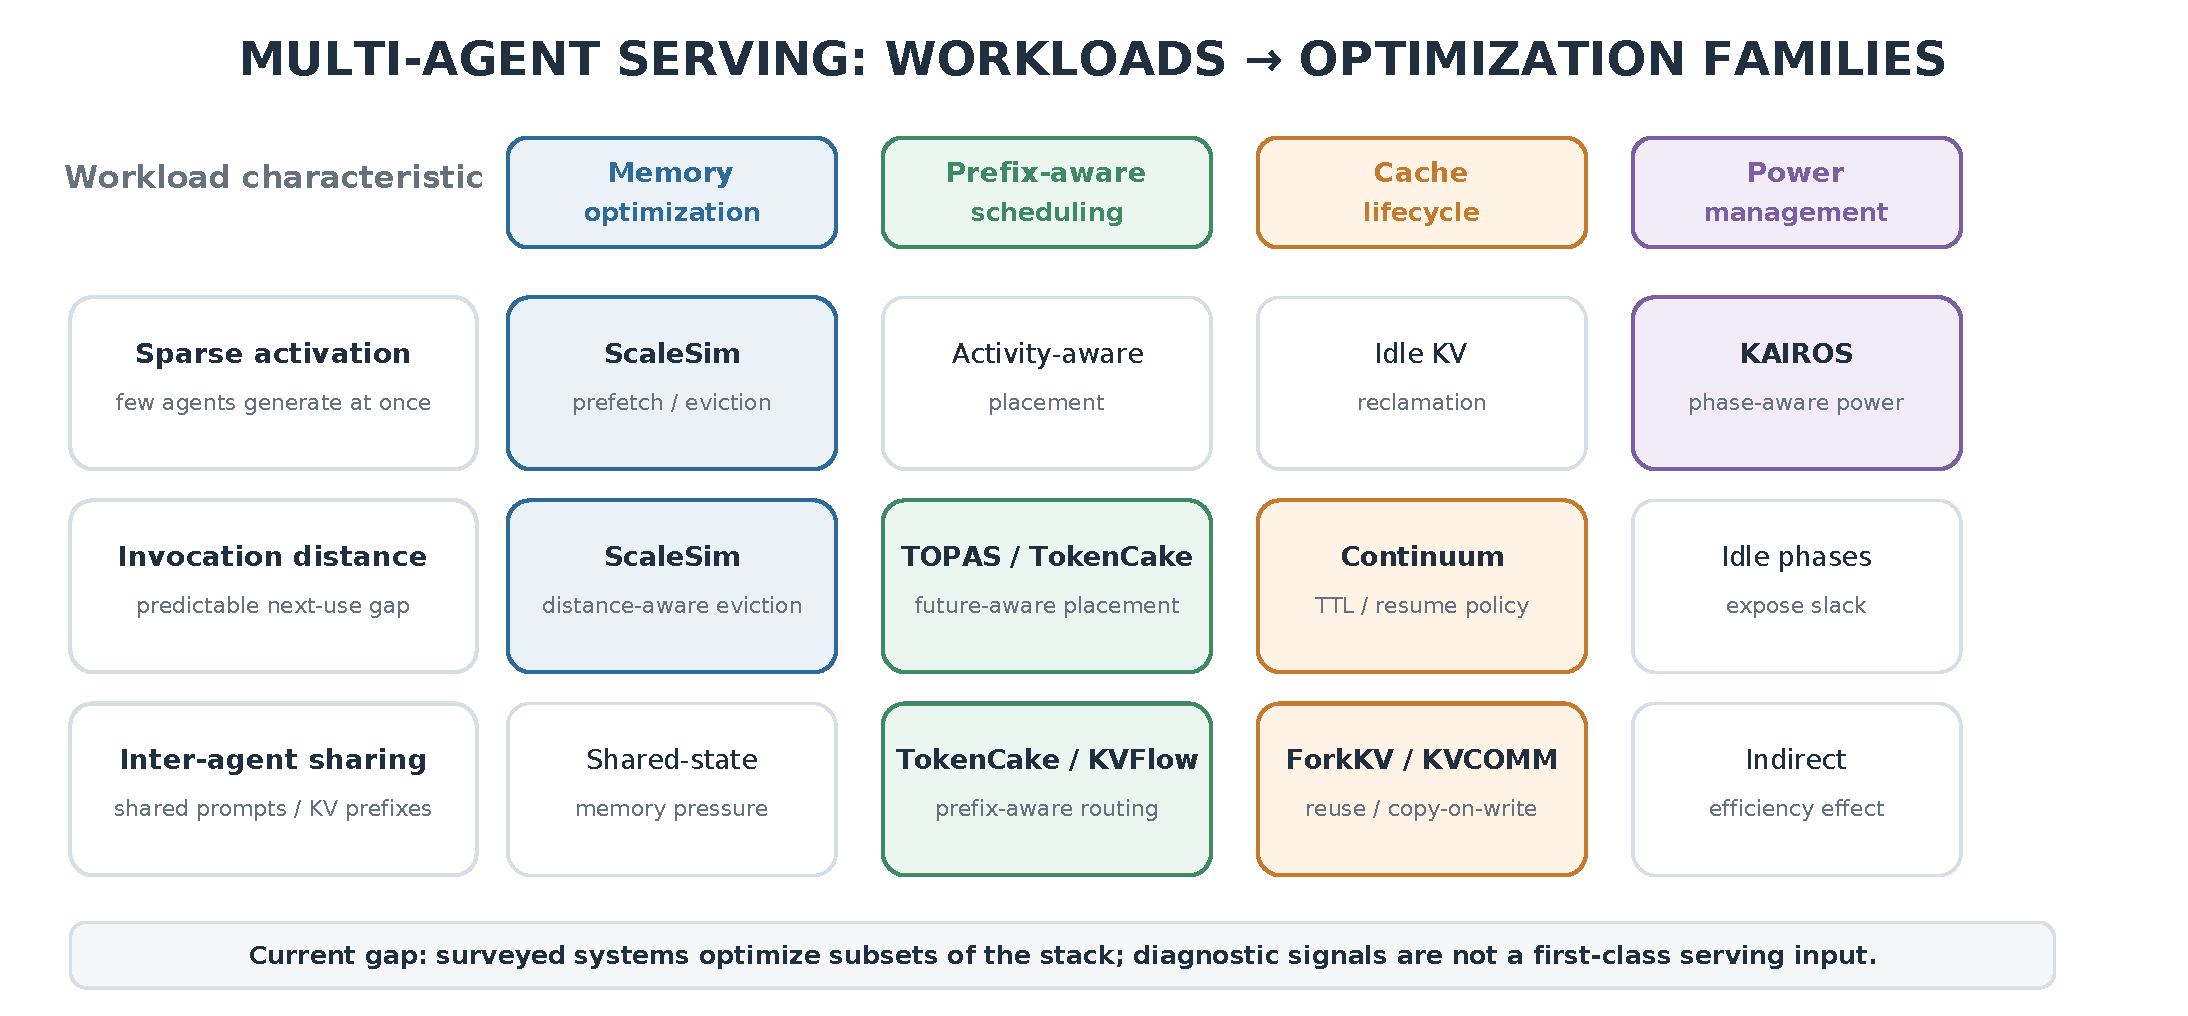
\includegraphics[width=\textwidth]{fig4_infrastructure.pdf}
\caption{Multi-agent serving challenges and optimization axes. Three workload characteristics (sparse activation, invocation distance, and inter-agent memory sharing, shown as shared prefixes in the figure) are exploited predictively by four families of application-aware systems spanning memory optimization, prefix-aware scheduling, cache lifecycle, and power management. No existing system jointly optimizes all four axes.}
\label{fig:infra_axes}
\end{figure*}

\section{The Diagnostics--Infrastructure Tension}\label{sec:tension}
The two layers surveyed so far are usually discussed as independent engineering problems. They are not: both place requirements on the same runtime state, and those requirements pull in opposite directions. Diagnostics needs state to be \emph{retained} long enough to explain a failure; serving infrastructure needs it \emph{discarded} quickly enough to serve the next request. The organising axis is therefore \emph{retention}, not timing: serving systems choose a retention policy with no regard for what diagnosis will need, and diagnosis, online or after the fact, must work from whatever survives. By the time an explanation is produced the discarded state is already gone, so the question is what the policy kept, not when the diagnosis ran.

The clearest evidence is a measurement rather than an argument. TraceElephant reports the same attribution task under two observability settings, and the gap is large: under the All-at-Once protocol, complete traces raise agent-level accuracy from 51\% to 62.2\%, and step-level accuracy from 16\% to 28.1\% (a 76\% relative gain)~\citep{traceelephant2026}. Output-only traces are not a failure of instrumentation; they are what a cheap-capture policy produces, because capturing every observation at every step is expensive to store and ship. That measured 76\% relative drop in step-level attribution is therefore the price of a retention decision, and it is a diagnostic cost no serving system currently accounts for.

\begin{figure*}[t]
\centering
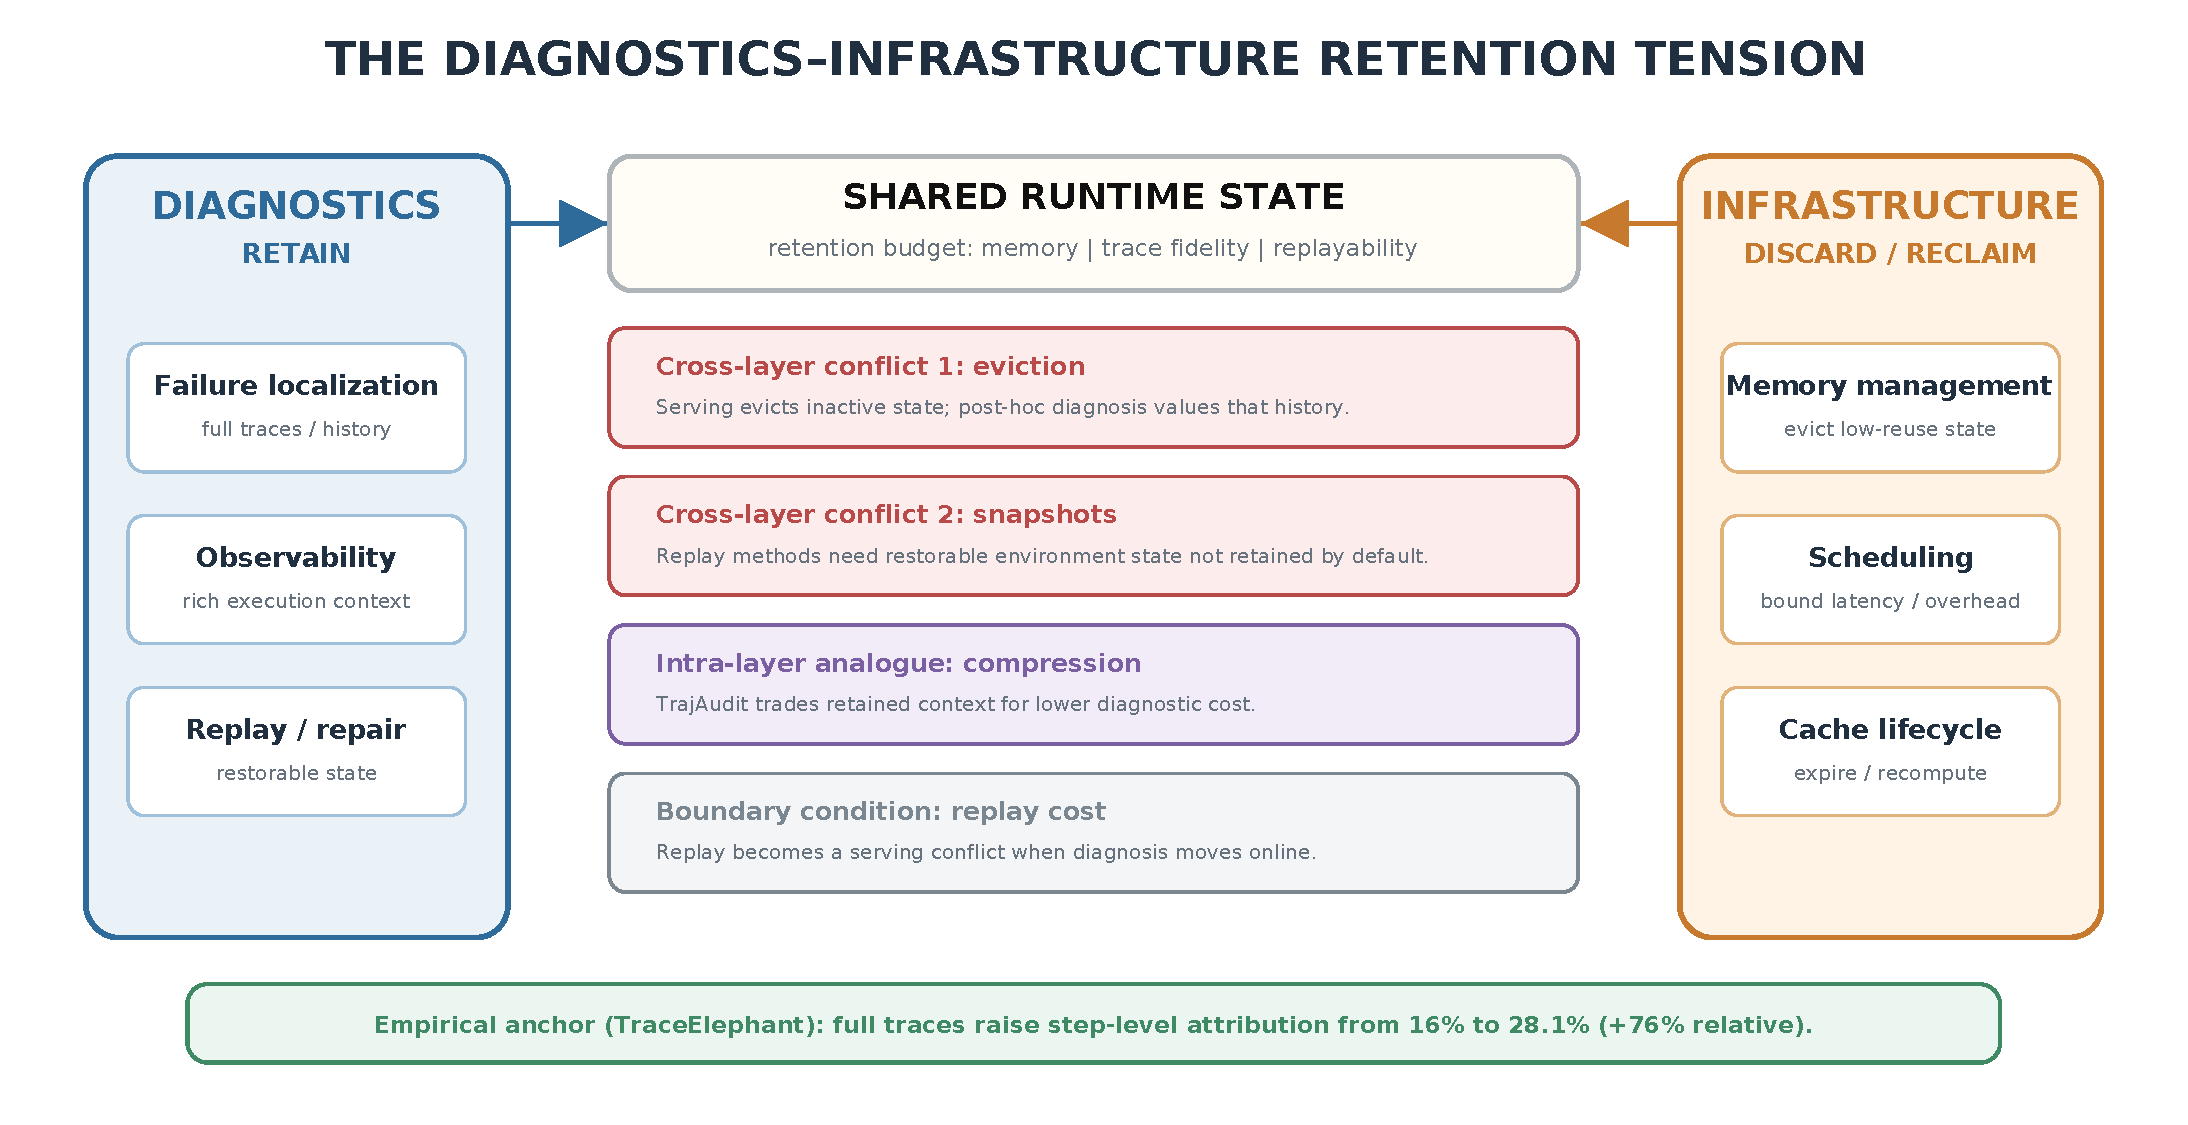
\includegraphics[width=\textwidth]{fig5_tension.pdf}
\caption{The diagnostics--infrastructure retention tension. The diagnostics layer (left) requires runtime state to be \emph{retained} for failure explanation, while the infrastructure layer (right) requires it to be \emph{discarded} for fast service. Two cross-layer conflict mechanisms, one intra-layer analogue, and one boundary condition act on shared runtime objects (centre). No existing system manages the retention budget as a first-class resource.}
\label{fig:tension}
\end{figure*}

We call this the diagnostics--infrastructure retention tension. It is not merely a matter of engineering effort left undone: the two layers optimise against different objectives on the same resource, so a policy that is optimal for one is close to anti-optimal for the other. Two cross-layer mechanisms make the conflict concrete; a third instance shows the same shape within the diagnostic layer itself; and a fourth marks where the conflict would become acute for online diagnosis.

\emph{Swapping state off the fast path.} ScaleSim's distance-aware eviction~\citep{zhou2026} selects the agent states with the longest invocation distance and moves them out of GPU memory, which is, from the diagnostics side, the set of inactive agents whose state a post-hoc attribution method would need in order to reconstruct the failure. The serving engine does not delete this state; it swaps it to host memory or storage. The retention question is therefore not whether the swap happens but whether the swapped-out state is reclaimed before diagnosis reads it, and whether the KV-cache is preserved or dropped and recomputed. A policy that is optimal under a memory budget makes the diagnostic copy the first candidate for reclamation, which is the conflict in its precise form.

\emph{Environment snapshots are not retained.} Replay-based attribution needs more than a text trace. FAMAS~\citep{famas2025} re-executes a failed task $k=20$ times and expects the environment to reach comparable states, and DoVer~\citep{dover2026} intervenes mid-trajectory and reruns from the intervention point, which requires the environment to be restorable. Serving infrastructure has no reason to retain environment snapshots, since they are not needed to schedule the next request. This is the concrete resource the replay-class methods lack, and it explains why they are evaluated on fixed corpora where the environment can be reconstructed offline rather than on live serving paths.

\emph{The diagnostic layer has an isomorphic tradeoff internally.} TrajAudit's Semantic Saliency Folding~\citep{trajaudit2026} compresses 86--92\% of observations into placeholders to fit the model's context window. This is the diagnostician's own retention decision, with more context yielding better attribution and less yielding lower cost. It is not cross-layer tension but a same-shaped problem inside one layer, and we note it because it shows the accounting question is not specific to serving.

\emph{Replay is a serving cost: a boundary condition.} The boundary flagged here is the replay budget itself, which is a separate concern from the restorable environment the previous instance requires: a method could hold a restorable environment and still replay once. FAMAS's twenty replays conflict with serving only if diagnosis runs on the serving path. FAMAS is an offline method evaluated on a fixed corpus, so for this instance the conflict is latent rather than actual: it marks where the tension would become acute, namely for any diagnostic that must run online. We therefore treat replay as the boundary condition of the retention argument rather than as a fourth mechanism. The existence of zero-replay debugging~\citep{zeroreplay2026} is indirect evidence that the cost is real when diagnosis is placed on the serving path.

Table~\ref{tab:tension} contrasts the two layers along the dimensions that generate these conflicts. The rows are not independent: retention budget is the shared resource, and every mechanism above is a different way of spending it. No surveyed system treats retention as a managed quantity, and the four co-design directions that follow from this view are developed in \S\ref{sec:discussion}.

\begin{table*}[t]
\centering
\caption{The diagnostics--infrastructure tension along shared runtime resources.}
\label{tab:tension}
\footnotesize
\setlength{\tabcolsep}{5pt}
\begin{tabular}{@{}p{0.20\textwidth}p{0.34\textwidth}p{0.34\textwidth}@{}}
\toprule
\textbf{Dimension} & \textbf{Diagnostics requirement} & \textbf{Infrastructure requirement} \\
\midrule
Runtime state & Full per-step inputs, outputs, and tool logs & Only what is needed to schedule the next request \\
Retention horizon & Retain until diagnosis completes & Discard as soon as reuse probability drops \\
Eviction criterion & Keep low-reuse-probability states & Evict low-reuse-probability states first \\
Granularity & Step-level and cross-agent (to localise cause) & Request- and agent-level (to place work) \\
Overhead budget & Tolerates replay and rich capture & Bounded by serving SLO; overhead is waste \\
Replay resources & Restorable environment snapshots & None retained \\
\bottomrule
\end{tabular}
\end{table*}
\vspace{-2pt}
{\footnotesize \emph{Observed instances.} Cross-layer: ScaleSim's eviction swaps (not deletes) the state a later diagnosis would need~\citep{zhou2026}; serving retains no environment snapshots needed by replay-based attribution~\citep{famas2025,dover2026}. Intra-layer analogue: TrajAudit compresses 86--92\% of observations~\citep{trajaudit2026}. Boundary: replay ($k{=}20$) is affordable only offline~\citep{famas2025}. Continuum's TTL expiry~\citep{continuum2025} raises resumption cost within the cache layer, not across the diagnostics--infrastructure boundary. Output-only capture costs 76\% relative step-level attribution accuracy~\citep{traceelephant2026}.}

\section{Discussion}\label{sec:discussion}
This survey has treated diagnostics and infrastructure as two bodies of work and, in \S\ref{sec:tension}, as two sets of requirements acting on the same runtime objects. This section discusses why the two developed separately, where the field disagrees with itself, what remains unsolved, and what a research agenda grounded in the tension would look like.

\paragraph*{Why the two layers were studied separately.}
The separation is largely sociological rather than technical. Diagnostics draws on two communities that rarely meet: the software engineering fault-localization and testing community (ICSE, ASE, FSE), where the unit of analysis is an execution trace, and the machine-learning community that publishes at ICLR, ICML, NeurIPS, and ACL. In our own reference set the ML side dominates, with only a minority of diagnostic papers (for example FALAT, AgentRx, and MASPrism) appearing at software-engineering venues. Neither community publishes at systems venues, which is where the serving work lives. Infrastructure grew out of systems and architecture (OSDI, SOSP, MLSys), where the unit is a request and the goal is throughput and latency under a resource budget. The two communities show little overlap in our own bibliography. This is an observation about the surveyed set, not a measured co-citation count: none of the serving systems in \S\ref{sec:infrastructure} evaluates against a diagnostic benchmark, and among the failure-localization methods in \S\ref{sec:diag_fl} the three paradigms matured with minimal cross-citation. The budgets differ too: a diagnostics paper can afford twenty replays per failure because it runs offline on a fixed corpus, while a serving paper treats any per-request overhead above single-digit percentages as unacceptable. This is why the tension we identified is not visible from within either community: each has optimized against a constraint the other does not face.

\paragraph*{Contested questions.}
Several genuine disagreements cut across the literature, and our evidence bears on each.

\emph{Should attribution be statistical, reasoning-based, or learned?} The three paradigms in \S\ref{sec:diag_fl} embody different bets. Statistical approaches assume failures leave a reproducible signature across replays; reasoning-based approaches assume a sufficiently capable model can infer the cause from a single trace; learned approaches assume the mapping is stable enough to be trained. The paradigms developed independently, which is either a healthy division of labour, with different regimes favouring different methods, or a duplication problem, in which three communities solve the same task with incompatible evaluation. Our evidence is equivocal. The paradigms do report on overlapping benchmarks now (Who\&When recurs across the statistical, reasoning, and learned families), which suggests convergence is beginning; but they still disagree about what an acceptable input cost is, so their headline numbers are not commensurable. We regard this as an open question rather than a settled one.

\emph{Should trace richness be maximized or minimized?} Diagnostics wants richer traces: TraceElephant's central result is that observability materially changes what can be attributed, with step-level accuracy far more sensitive than agent-level~\citep{traceelephant2026}. Serving wants cheaper traces: the same paper's output-only setting is not a failure of instrumentation but the natural consequence of capturing only what is cheap to keep. Both positions are defensible, and the field has not agreed on where the line sits. The absence of a standard for \emph{what must be retained} (as opposed to what may be captured) is the clearest symptom.

\emph{Is retention an engineering detail or an architectural resource?} Current systems treat retention as a local policy: an eviction rule inside a serving engine, a TTL chosen per workload. Under this framing, diagnostics is simply a consumer that must cope with whatever survives. The alternative, which we favour and which \S\ref{sec:tension} argues for, is that retention is a first-class resource shared between layers, with an explicit budget and explicit trade-offs. Nothing in the current literature settles this; no system reports retention as a managed quantity.

\emph{Should safety intervene proactively or reactively?} The safety paradigms in \S\ref{sec:diag_safety} disagree about when a guardrail should act. Topology-based and policy-verification methods examine a proposed action before it executes; reactive and recovery-oriented methods intervene after detection. The disagreement is substantive rather than stylistic, because the two positions have opposite implications for the tension. A proactive guardrail must hold enough state about the proposed action to judge it, which means retaining execution context that a serving engine would rather evict; a reactive guardrail tolerates a window during which damage may already have propagated through the communication graph. The literature reports both kinds of system as successful, but not on a common workload with a common overhead budget, so the choice between them remains an empirical question. That the field has not settled it is unsurprising given that, as we noted above, no benchmark measures the serving cost of a guardrail at all.

\paragraph*{The safety layer as a third constraint.}
Safety is often filed under diagnostics, and we have followed that convention in our taxonomy, but the tension analysis suggests it behaves differently from either layer. A guardrail is not a passive consumer of traces, like an attribution method, nor a pure resource manager, like a scheduler. It is a component that must inspect runtime state \emph{and} act on the serving path, which places it under both constraints at once: it needs the retention that diagnostics needs in order to judge an action, and it must meet the latency budget that infrastructure meets in order to act in time. Multi-agent settings sharpen this, because the object a guardrail must reason about is not a single agent's state but the communication graph spanning all of them, the same graph whose maintenance cost a serving system is trying to control. We regard the placement of safety within the two-layer picture as genuinely unsettled: treating it as a subcategory of diagnostics, as the prevailing convention does, may understate the scheduling burden it imposes.

\paragraph*{Fundamental concepts and open problems.}
The organising problem is the retention--discard conflict. Diagnostics needs runtime objects to persist until a failure is explained; serving needs them gone as soon as their reuse probability drops. Two cross-layer mechanisms make the conflict concrete (Table~\ref{tab:tension}): eviction swaps agent state off the fast path at the moment a later diagnosis would need it, and serving retains no environment snapshots, so replay-based attribution must reconstruct them offline. A third instance, TrajAudit's trace compression, shows the same shape within the diagnostic layer itself. A fourth, replay cost, marks where the conflict would become acute for any diagnostic that must run on the serving path.

Framed this way, the open problem is an accounting one. A principled treatment would make retention a budgeted quantity, allocated per agent and per trajectory, priced against serving objectives, and released on a schedule rather than by a local eviction heuristic. No published system does this. The nearest analogues are cache-retention policies, which optimise for reuse probability and therefore systematically discard precisely the low-probability states that post-hoc diagnosis prizes. We note that this framing is a proposal, not a result: it follows from the behaviours we verified in the surveyed systems, but no experiment in the literature tests it directly.

\paragraph*{Research gaps.}
Three gaps follow from the above and are, in our reading, the field's most tractable openings. First, \emph{no benchmark measures diagnostics--infrastructure interaction}. Every benchmark surveyed in \S\ref{sec:diag_bench} evaluates attribution quality on a fixed corpus; none measures attribution quality under a realistic serving policy, nor the serving cost of achieving a given diagnostic fidelity. The interaction is therefore unmeasured in both directions. Second, \emph{no standard specifies what must be retained}. OpenTelemetry conventions~\citep{opentelemetry2026} and structured-logging proposals~\citep{agenttrace2026} standardise capture, not retention, so interoperability breaks exactly when a failure is investigated. Third, \emph{evaluation scale is mismatched}. Diagnostics methods are validated on tens to hundreds of failures (FAMAS: 82; TraceElephant: 220; the largest telemetry study we found: 275 executions~\citep{whenfail2026}), while production systems execute thousands of tasks per hour. Whether the reported accuracies survive that scale is untested, and the retention costs that would be required to make them survive are unreported.

\paragraph*{Evidence and its limits.}
Two methodological choices shape what this survey can claim, and both are recorded here because they bound how the results should be read. The first is the verification strategy described in \S\ref{sec:background}. Its consequence is uneven depth. The failure-localization and infrastructure layers contain the systems we could verify against full text, and they carry the quantitative analysis; the observability and safety layers rest substantially on abstract-level evidence, and we have accordingly described what those systems do without ranking them. Readers should treat the two halves of our taxonomy as carrying different evidential weight, which Table~\ref{tab:obs_safety} and Table~\ref{tab:failure_loc} make visible through their tier and publication-type columns.

The second is the recency of the field. A large fraction of the surveyed work (by our count, roughly two-thirds of the cited systems) appears as preprints without a confirmed venue, and several entries carry 2026 dates. This is a property of a fast-moving area rather than a defect of any individual work, but it bounds our conclusions in a specific way: venue-independent claims, such as the existence of the retention--discard conflict, are robust to it, whereas any statement about which method currently performs best is not, because the ranking can change between preprint revisions. We have therefore avoided ranking language throughout and reported matched comparisons only where the source supports them.

\paragraph*{Broader impact.}
The retention question has a privacy dimension that sits alongside its performance dimension. Diagnostics requires retaining execution state, and that state routinely contains user inputs, tool outputs, and reasoning traces; richer retention therefore extends the lifetime of potentially sensitive data. Infrastructure optimisations that predict agent activation introduce a second concern, since an accurate model of when agents will act is also a model of what agents are doing, and could be repurposed for monitoring beyond the operational purpose it was built for. We see no technical mechanism that separates these uses once the state is retained; the practical mitigations are policy-level (bounded retention windows, access control, and audit trails for production deployments~\citep{auditableagents2026}), and they trade away some of the diagnostic fidelity that motivates retention in the first place. This is a genuine cost of the research direction we advocate, and it should be weighed explicitly when retention budgets are designed rather than after the fact.

\paragraph*{Limitations.}
Beyond the evidential asymmetry noted above, five limitations bound this review. First, our infrastructure analysis rests on ScaleSim as a full-text case study, with TokenCake, Continuum, and KAIROS examined at the abstract level; the tension in \S\ref{sec:tension} is argued from the verified behaviour of these components rather than from a purpose-built experiment, and would be strengthened by direct measurement of diagnostic accuracy under real serving policies. Second, the third workload characteristic of contribution~2 (inter-agent memory sharing) is likewise characterised at the abstract level, so the systems cited under it are enumerated rather than compared. Third, the survey lacks a formal search methodology: we did not run a registered protocol with predefined databases, query strings, date windows, or screening criteria, so the system and reference set should be read as a curated landscape rather than as the output of a reproducible search, and a systematic review with PRISMA-style reporting would likely surface additional systems. Fourth, the safety discussion draws on venue-published work (G-Safeguard at ACL, ShieldAgent at ICML) alongside preprints read at abstract level; the former were verified through their published text but without page-level cross-checking of every reported number. Fifth, our taxonomy is descriptive of what has been built, not predictive of what should be: where we identify an absent capability, such as retention accounting, we are reporting a gap in the literature rather than asserting that no unpublished system has closed it. Our verification strategy trades quantitative breadth for citation honesty, and these limitations mark where that trade is most visible. We note that citing preprints does not breach the journal's policy on unpublished material, which concerns unpublished original data rather than public preprints of reviewed work.

\begin{figure*}[t]
\centering
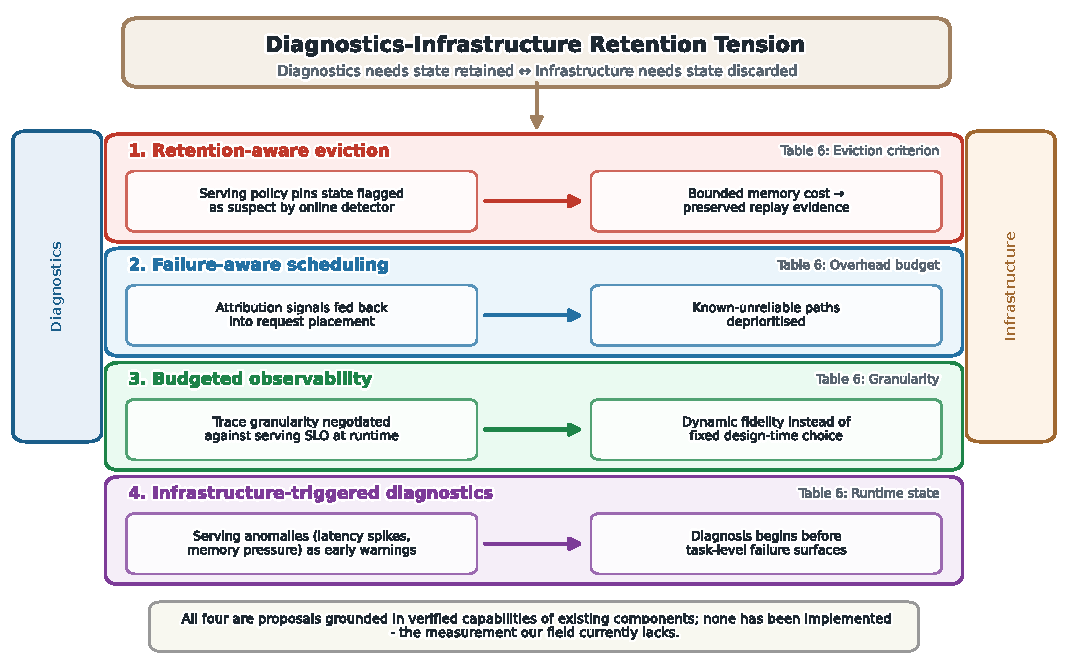
\includegraphics[width=\textwidth]{fig6_codesign_agenda.pdf}
\caption{Co-design research agenda derived from the diagnostics--infrastructure tension. Four directions address specific rows of Table~\ref{tab:tension}: retention-aware eviction, failure-aware scheduling, budgeted observability, and infrastructure-triggered diagnostics. Each converts a tension point into a concrete research challenge at the boundary between the two layers.}
\label{fig:codesign}
\end{figure*}

\paragraph*{Future development.}
The four co-design directions introduced in \S\ref{sec:tension} and developed here form a research agenda rather than a list of features, because each addresses a specific row of Table~\ref{tab:tension}. \emph{Retention-aware eviction} would let a serving policy pin the state that an online detector flags as suspect, converting a bounded memory cost into preserved replay evidence. \emph{Failure-aware scheduling} would feed attribution signals back into request placement, so that known-unreliable execution paths are deprioritised. \emph{Budgeted observability} would negotiate trace granularity against the serving SLO at runtime instead of fixing it at design time. \emph{Infrastructure-triggered diagnostics} would treat serving anomalies such as latency spikes and memory pressure as early-warning signals that begin diagnosis before the task-level failure surfaces. We stress that all four are proposals grounded in the verified capabilities of existing components; none has been implemented, and each would need to demonstrate that the serving cost it incurs is repaid by diagnostic gains, the measurement our field currently lacks.

\section{Conclusion}\label{sec:conclusion}
Foundation model-based multi-agent systems now execute production workloads whose reliability depends on two layers that the research community has built separately: diagnostics, which explains failure after the fact, and infrastructure, which keeps serving efficient in the moment. This review has assembled both into a single taxonomy: four diagnostic subcategories spanning three failure-localization paradigms and three safety paradigms, and four infrastructure optimization axes spanning memory optimization, prefix-aware scheduling, cache lifecycle, and power management. It has compared the reviewed systems quantitatively where the evidence permits, holding publication type and verification tier explicit throughout.

The central argument is that these layers are not independent. They act on the same runtime objects under opposed objectives: diagnostics must retain state long enough to explain a failure, while serving infrastructure must discard it as soon as reuse becomes unlikely. We have shown that this tension is already visible in two cross-layer mechanisms and an intra-layer analogue that hold for post-hoc diagnosis, with a boundary condition marking where it would become acute online, and that no surveyed system accounts for retention as a managed resource. Treating retention as a shared, budgeted resource, rather than a local eviction heuristic, is we argue the problem that connects the two layers and the most promising direction for the work that follows. The taxonomy, the verified comparisons, and the tension analysis presented here are offered as a common frame for that effort.


\section*{Conflict of Interest Statement}
The authors declare that the research was conducted in the absence of any commercial or financial relationships that could be construed as a potential conflict of interest.

\section*{Author Contributions}
Author 1: conceptualization, methodology, literature search and analysis, writing, and revision. Author 2: literature search, data curation, figure generation, and writing. Author 3: supervision, critical review, and project administration. All authors contributed to the article and approved the submitted version.

\section*{Funding}
This research received no external funding.

\section*{Data Availability Statement}
This is a literature survey covering 112 references and 45 systems (counted across the survey's own system tables, excluding benchmarks and comparator surveys), with 6 figures and 6 tables. No new data were generated or analyzed in this study; all reviewed literature is publicly available from the cited sources.

\section*{Ethics Statement}
This survey reviews published systems and introduces no new experimental subjects or datasets, but it advocates a research direction whose costs are ethical as well as technical. Diagnostics requires retaining execution state, which routinely contains user inputs, tool outputs, and reasoning traces, so richer retention extends the lifetime of potentially sensitive data; infrastructure optimizations that predict agent activation could likewise be repurposed for monitoring. We see no technical mechanism that separates these uses once state is retained, and recommend bounded retention windows, access control, and audit trails, weighed explicitly against the diagnostic fidelity that retention buys.

\section*{AI Use Disclosure}
This manuscript was prepared with AI-assisted tools. Specifically, an AI research assistant (Apex Research) was used for four tasks: literature search and screening, taxonomy construction, draft generation, and reference verification. Quantitative claims used for cross-system comparison were verified through full-text analysis of primary sources; results marked [a] are reported as stated in source abstracts. The specific generative-AI prompts used are listed in the Supplementary Material. The authors reviewed and approved all AI-assisted output and take full responsibility for the content, accuracy, and completeness of the manuscript.

\section*{Acknowledgements}
The authors acknowledge the use of the AI-assisted tools detailed in the AI Use Disclosure above.

\section*{Supplemental Data}
The Supplementary Material for this article contains the list of generative-AI prompts used in manuscript preparation, per the Frontiers BE WISE AI guidance.

\bibliographystyle{Frontiers-Harvard}
{\small
\bibliography{references}
}

\end{document}
